\section{1174054 - Aulyardha Anindita}

\subsection{Teori}
\begin{enumerate}
\item Random Forest \\
Random Forest adalah salah satu metode yang ada di Decision Tree. Decision Tree yaitu suatu diagram atau yang biasa dikenal dengan pohon pengambil keputusan merupakan suatu diagram alir yang memiliki bentuk seperti pohon yang digunakan untuk mengumpulkan data atau root node. Random Forest dapat juga diartikan sebagai kombinasi dari setiap tree yang kemudian dikombinasikan dalam suatu model yang bergantung pada sebuah nilai vektor random dari distribusi yang sama pada semua tree yang masing-masing memiliki descision tree tergantung dari kedalaman yang maksimal.

Random Forest juga merupakan algoritma yang biasa digunakan untuk megklasifikasikan data dalam jumlah yang besar. klasifikasi tersebut dilakukan dengan penggabungan pohon yang akan mempengaruhi akurasi yang didapatkan.

\begin{figure}[H]
		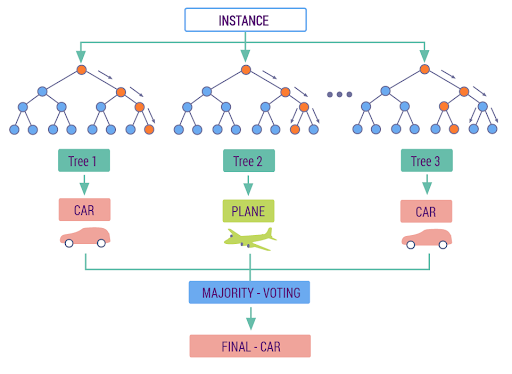
\includegraphics[width=4cm]{figures/1174054/3/1.png}
		\centering
		\caption{Random Forest}
\end{figure}

\item Cara Membaca Dataset \\
\begin{itemize}
\item Untuk langkah pertama, kita mendownload terlebih dahulu file dataset nya, disini saya mengambil dataset burung yang ada pada teori
\item Setelah download selesai, buka software spyder untuk melihat isi dari file dataset yang telah kita download
\item Isi dari data tersebut memiliki extensi file yang bernama .txt yang didalamnya terdapat class dari field.
\item Contohnya pada data jenis burung memiliki file index dan angka, dimana index tersebut berisi angka yang memiliki arti jenis burung dan nama burung
\item Sedangkan pada field memiliki isi nilai yang berupa 0 dan 1 dimana memiliki sifat boolean yaitu true or false
\item Hal ini terjadi karena komputer hanya bisa membaca bilangan biner sehingga field tersebut berupa angka, angka yang dimaksud disini adalah angka 0 yang berarti false dan angka 1 yang berarti true
\end{itemize}

\item Cross Validation \\
Cross Validation (CV) merupakan suatu metode statistik yang digunakan untuk mengevaluasi kinerja model atau algoritma dengan cara data dipisahkan menjadi dua subset yaitu data proses pembelajaran dan data validasi atau evaluasi. suatu model atau algoritma tersebut dilatih oleh subset untuk pembelajaran kemudian divalidasi oleh subset validasi. sehingga pemilihan jenis cross validation dapat didasarkan pada ukuran dataset, biasanya cross validation k-fold berguna untuk mengurangi waktu komputasi dengan menjaga keakuratan estimasi. Tujuan dari cross validation yaitu untuk mendefinisikan dataset guna menguju dalam fase pelatihan untuk membatasi masalah seperti overfitting dan underfitting serta mendapatkan wawasan tentang bagaimana model akan digeneralisasikan ke set data independen.

\item Arti score 44 \% pada random forest, 27\% pada decision tree dan 29 \% dari SVM. \\
Scrore 44 \% diperoleh dari hasil pengolahan dataset jenis burung. Hal ini dilakukan untuk proses pembagian data testing dan data training kemudian diproses dan menghasilkan score sebanyak 44 \% yang artinya bahwa score tersebut digunakan sebagai pembanding dalam tingkat keakuratannya.

Pada Decision Tree memperoleh data yang lebih kecil yaitu sebanyak 27 \% hal ini disebabkan karena data yang diolah menggunakan decision tree dibagi menjadi beberapa tree, sehingga dapat disimpulkan hal ini dilakukanuntuk mendapatkan data yang akurat.

Pada SVM memperoleh score sebanyak 29 \% hal ini disebabkan karena data yang dimiliki masih bernilai netral sehingga tingkat keakuratannya masih belum jelas.

\item Cara Membaca Confusion Matriks\\
Untuk membaca confusion matriks dapat menggunakan source code sebagai berikut :
\lstinputlisting[firstline=233, lastline=237]{src/1174054/3/1174054_teori.py}
\hfill\break
Dimana numpy akan mengurus semua data yang berhubungan dengan matrix. Pada source code tersebut digunakan dalam melakukan read pada dataset burung dengan menggunakan metode confusion matrix. Dalam confusion matrix terdapat 4 istilah yaitu True Positive yang merupakan data positif yang terdeteksi benar, True Negatif yang merupakan data negatif akan tetapi terdeteksi benar, False Positif merupakan data negatif namun terdeteksi sebagai data positif, False Negatif merupakan data posotif namun terdeteksi sebagai data negatif. Adapun contoh hasil read dataset menggunakan confusion matrix dapat dilihat dibawah ini :
	\begin{figure}[H]
	\centering
		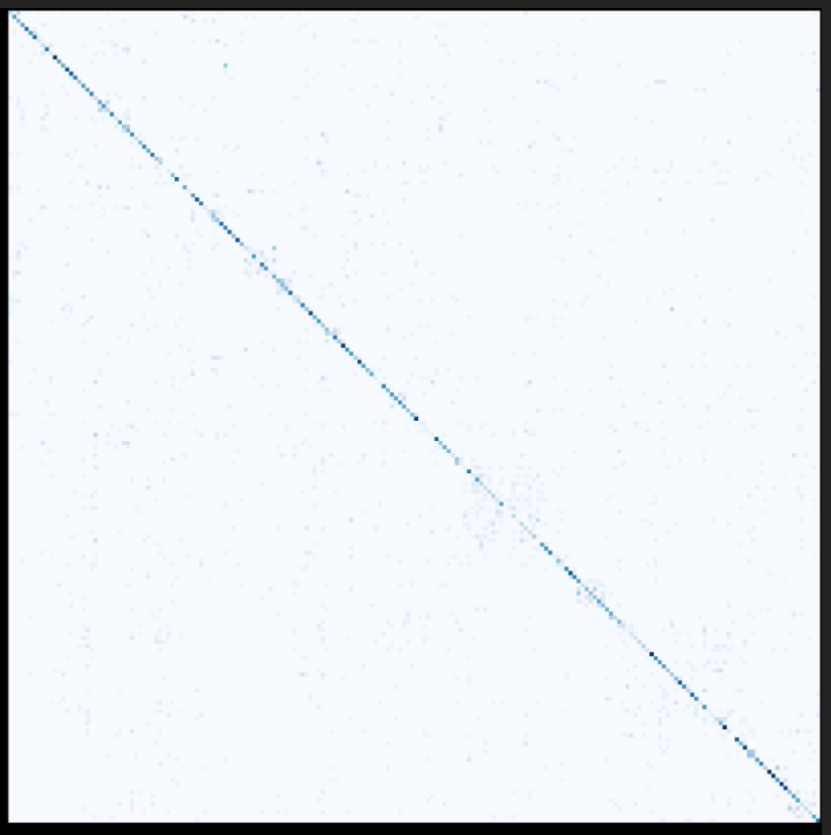
\includegraphics[width=2cm]{figures/1174054/3/2.png}
		\caption{Confusion Matriks}
	\end{figure}

\item Voting pada random forest \\
Voting pada random forest ialah sebuah proses pemilihan dari tree yang dimana akan dimunculkan hasilnya dan disimpulkan menjadi informasi yang pasti. Untuk lebih jelasnya saya akan memberikan sebuah contoh bagaimana voting bekerja : 
	\begin{figure}[H]
	\centering
		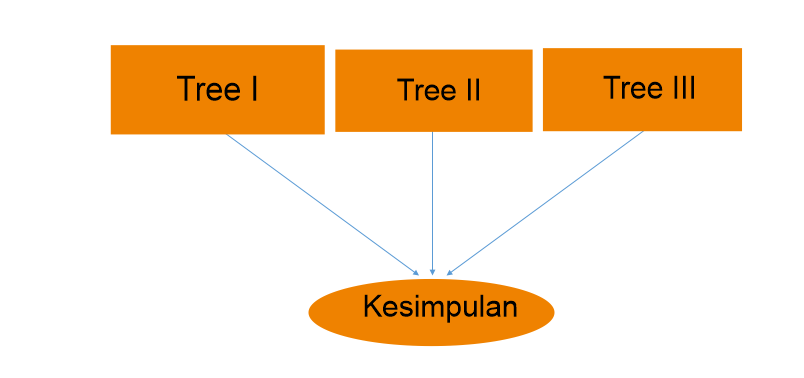
\includegraphics[width=4cm]{figures/1174054/3/3.png}
		\caption{Decision Tree.}
	\end{figure}
Dimana ditunjukkan pada gambar diatas terdapat 3 tree. Dalam tree tersebut akan dilakukan proses voting. Saya akan memberikan contoh kasus, dimana akan diadakan voting untuk menentukan sebuah hp. Dalam tree akan diberikan sejumlah data misalnya saja data tersebut berupa gambar, yang dimana data tersebut akan dipilih dengan cara voting. Hasil voting akhir dari setiap tree menunjukkan hp vivo, yang berarti kesimpulan dari data yang telah diberikan menyatakan gambar tersebut adalah hp vivo. Bagaimana apabila terjadi perbedaan data misalnya saja pada tree 1 dan 2 menyatakan hp vivo sedangkan pada tree 3 menyatakan hp oppo, maka kesimpulan yang di ambil adalah hp vivo dikarenakan hasil voting terbanyak adalah hp vivo.
\end{enumerate}

\subsection{Praktek}
\begin{enumerate}
\item Aplikasi Sederhana Menggunakan Pandas
\hfill\break
	\lstinputlisting[firstline=9, lastline=12]{src/1174054/3/1174054_praktek.py}
Hasilnya :
\begin{figure}[H]
		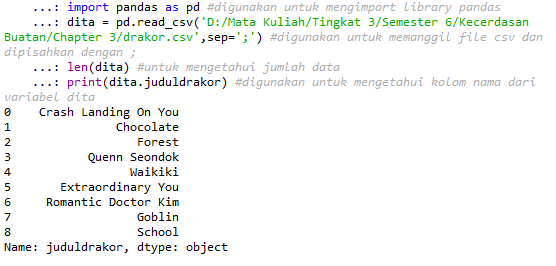
\includegraphics[width=4cm]{figures/1174054/3/4.png}
		\centering
		\caption{Hasil Nomor 1}
\end{figure}

\item Nomor 2
\hfill\break
	\lstinputlisting[firstline=13, lastline=16]{src/1174054/3/1174054_praktek.py}
Hasilnya :
\begin{figure}[H]
		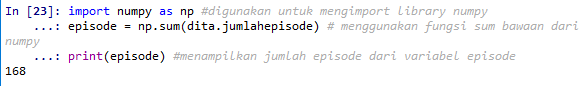
\includegraphics[width=4cm]{figures/1174054/3/5.png}
		\centering
		\caption{Hasil Nomor 2}
\end{figure}

\item Nomor 3
\hfill\break
	\lstinputlisting[firstline=17, lastline=35]{src/1174054/3/1174054_praktek.py}
Hasilnya :
\begin{figure}[H]
		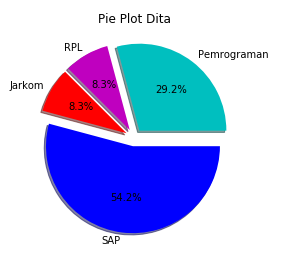
\includegraphics[width=4cm]{figures/1174054/3/6.png}
		\centering
		\caption{Hasil Nomor 3}
\end{figure}

\item Nomor 4
\hfill\break
\begin{itemize}
\item Source Code pertama pada random forest berfungsi untuk membaca dataset yang memiliki format text file dengan mendefinisikan variabel yang bernama imgatt. Variabel tersebut berisi value untuk membaca data. 
\lstinputlisting[firstline=10, lastline=14]{src/1174054/3/1174054_teori.py}
Hasilnya :
\begin{figure}[H]
	\centering
		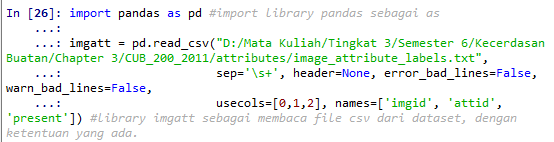
\includegraphics[width=4cm]{figures/1174054/3/7.png}
		\caption{Hasil Soal 4 - 1}
\end{figure}
		
\item Pada source code berikutnya akan mengembalikan baris teratas dari DataFrame variabel imgatt.
\lstinputlisting[firstline=19, lastline=19]{src/1174054/3/1174054_teori.py}
Hasilnya :
\begin{figure}[H]
	\centering
		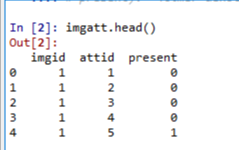
\includegraphics[width=4cm]{figures/1174054/3/8.png}
		\caption{Hasil Soal 4 - 2}
\end{figure}
		
\item Pada output berikutnya akan menampilkan jumlah kolom dan baris dari DataFrame imgatt. 
\lstinputlisting[firstline=24, lastline=24]{src/1174054/3/1174054_teori.py}
Hasilnya :
\begin{figure}[H]
	\centering
		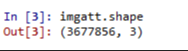
\includegraphics[width=4cm]{figures/1174054/3/9.png}
		\caption{Hasil Soal 4 - 3}
\end{figure}
		
\item Variabel imgatt2 telah menggunakan function yang bernama pivot guna mengubah kolom jadi baris dan sebaliknya dari DataFrame sebelumnya.
\lstinputlisting[firstline=29, lastline=29]{src/1174054/3/1174054_teori.py}
Hasilnya :
\begin{figure}[H]
	\centering
		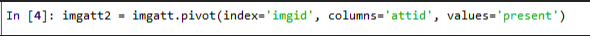
\includegraphics[width=4cm]{figures/1174054/3/10.png}
		\caption{Hasil Soal 4 - 4}
\end{figure}
		
\item Variabel imgatt2 head berfungsi untuk mengembalikan value teratas pada DataFrame imgatt2.
\lstinputlisting[firstline=34, lastline=34]{src/1174054/3/1174054_teori.py}
Hasilnya :
\begin{figure}[H]
	\centering
		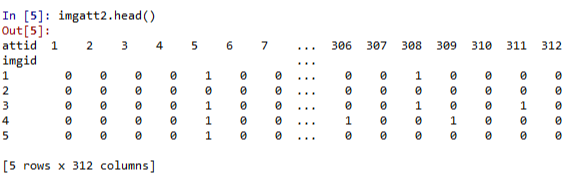
\includegraphics[width=4cm]{figures/1174054/3/11.png}
		\caption{Hasil Soal 4 - 5}
\end{figure}
		
\item Menghasilkan jumlah kolom dan baris pada DataFrame imgatt2.
\lstinputlisting[firstline=39, lastline=39]{src/1174054/3/1174054_teori.py}
Hasilnya :
\begin{figure}[H]
	\centering
		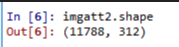
\includegraphics[width=4cm]{figures/1174054/3/12.png}
		\caption{Hasil Soal 4 - 6}
\end{figure}
		
\item Menunjukkan dalam melakukan pivot yang mana imgid menjadi sebuah index yang unik.
\lstinputlisting[firstline=44, lastline=47]{src/1174054/3/1174054_teori.py}
Hasilnya :
\begin{figure}[H]
	\centering
		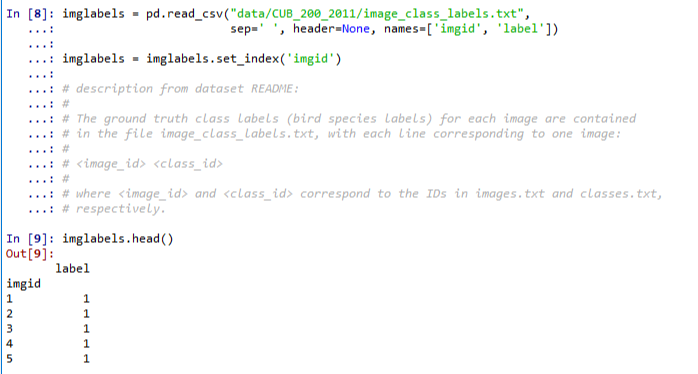
\includegraphics[width=4cm]{figures/1174054/3/13.png}
		\caption{Hasil Soal 4 - 7}
\end{figure}
		
\item Akan melakukan load jawabannya yang berisi apakah burung tersebut termasuk spesies yang mana. Kolom tersebut yaitu imgid dan label.
\lstinputlisting[firstline=52, lastline=52]{src/1174054/3/1174054_teori.py}
Hasilnya :
\begin{figure}[H]
	\centering
		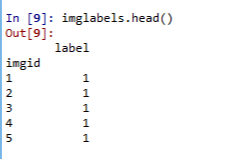
\includegraphics[width=4cm]{figures/1174054/3/14.png}
		\caption{Hasil Soal 4 - 8}
\end{figure}
		
\item Menunjukkan bahwa jumlah baris sebanyak 11788 dan kolom 1 yang dimana kolom tersebut adalah jenis spesies pada burung.
\lstinputlisting[firstline=57, lastline=57]{src/1174054/3/1174054_teori.py}
Hasilnya :
\begin{figure}[H]
	\centering
		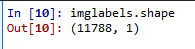
\includegraphics[width=4cm]{figures/1174054/3/15.png}
		\caption{Hasil Soal 4 - 9}
\end{figure}
		
\item Melakukan join antara imgatt2 dengan imglabels dikarenakan memiliki isi yang sama sehingga akan mendapatkan sebuah data ciri-ciri dan data jawaban sehingga bisa dikategorikan sebagai supervised learning.
\lstinputlisting[firstline=62, lastline=63]{src/1174054/3/1174054_teori.py}
Hasilnya :
\begin{figure}[H]
	\centering
		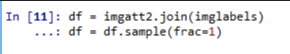
\includegraphics[width=4cm]{figures/1174054/3/16.png}
		\caption{Hasil Soal 4 - 10}
\end{figure}
		
\item Melakukan drop pada label yang ada didepan dan akan menggunakan label yang baru di joinkan.
\lstinputlisting[firstline=68, lastline=69]{src/1174054/3/1174054_teori.py}
Hasilnya :
\begin{figure}[H]
	\centering
		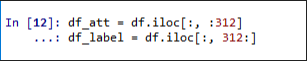
\includegraphics[width=4cm]{figures/1174054/3/17.png}
		\caption{Hasil Soal 4 - 11}
\end{figure}
		
\item Mengecek isi 5 data teratas pada df att.
\lstinputlisting[firstline=74, lastline=74]{src/1174054/3/1174054_teori.py}
Hasilnya:
\begin{figure}[H]
	\centering
		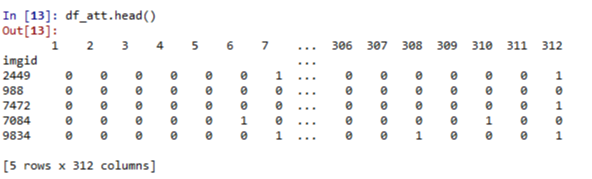
\includegraphics[width=4cm]{figures/1174054/3/18.png}
		\caption{Hasil Soal 4 - 12}
\end{figure}
		
\item Mengecek isi data teratas dari df label.
\lstinputlisting[firstline=79, lastline=79]{src/1174054/3/1174054_teori.py}
Hasilnya:
\begin{figure}[H]
	\centering
		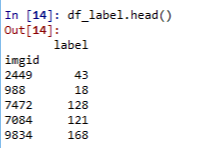
\includegraphics[width=4cm]{figures/1174054/3/19.png}
		\caption{Hasil Soal 4 - 13}
\end{figure}
		
\item Membagi 8000 row pertama menjadi data training dan sisanya adalah data testing.
\lstinputlisting[firstline=84, lastline=90]{src/1174054/3/1174054_teori.py}
Hasilnya:
\begin{figure}[H]
	\centering
		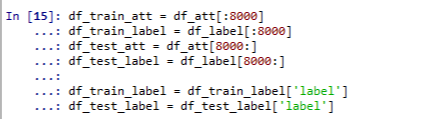
\includegraphics[width=4cm]{figures/1174054/3/20.png}
		\caption{Hasil Soal 4 - 14}
\end{figure}
		
\item Pemanggilan class RandomForestClassifier. Dimana artinya menunjukkan banyak kolom pada setiap tree adalah 50.
\lstinputlisting[firstline=95, lastline=96]{src/1174054/3/1174054_teori.py}
Hasilnya:
\begin{figure}[H]
	\centering
		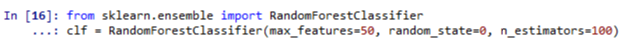
\includegraphics[width=4cm]{figures/1174054/3/21.png}
		\caption{Hasil Soal 4 - 15}
\end{figure}
		
\item Menunjukkan hasil prediksi dari Random Forest.
\lstinputlisting[firstline=101, lastline=101]{src/1174054/3/1174054_teori.py}
Hasilnya:
\begin{figure}[H]
	\centering
		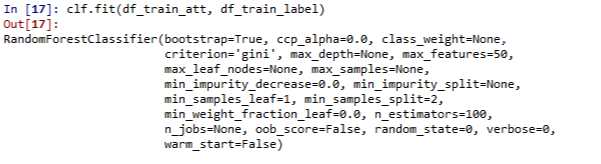
\includegraphics[width=4cm]{figures/1174054/3/22.png}
		\caption{Hasil Soal 4 - 16}
\end{figure}

\item Menampilkan besaran akurasi dari prediksi pada Random Forest yang merupakan score perolehan klarifikasi.
\lstinputlisting[firstline=106, lastline=106]{src/1174054/3/1174054_teori.py}
Hasilnya:
\begin{figure}[H]
	\centering
		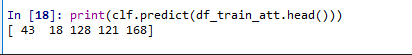
\includegraphics[width=4cm]{figures/1174054/3/23.png}
		\caption{Hasil Soal 4 - 17}
\end{figure}
\begin{figure}[H]
	\centering
		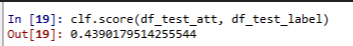
\includegraphics[width=4cm]{figures/1174054/3/24.png}
		\caption{Hasil Soal 4 - 17}
\end{figure}
\end{itemize}

\item Nomor 5
\hfill\break
\begin{itemize}
\item Melakukan import confusion matrix pada library sklearn matriks.
\lstinputlisting[firstline=116, lastline=118]{src/1174054/3/1174054_teori.py}
Hasilnya:
\begin{figure}[H]
	\centering
		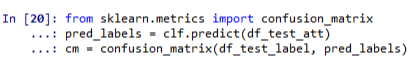
\includegraphics[width=4cm]{figures/1174054/3/25.png}
		\caption{Hasil Soal 5 - 1}
\end{figure}
		
\item Menampilkan isi cm dalam bentuk matrix yang berupa array.
\lstinputlisting[firstline=123, lastline=123]{src/1174054/3/1174054_teori.py}
Hasilnya:
\begin{figure}[H]
	\centering
		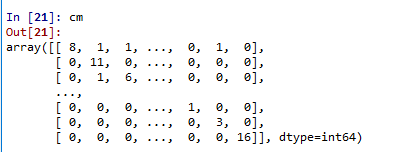
\includegraphics[width=4cm]{figures/1174054/3/26.png}
		\caption{Hasil Soal 5 - 2}
\end{figure}
		
\item Membuat dan menampilkan hasil plot.
\lstinputlisting[firstline=128, lastline=171]{src/1174054/3/1174054_teori.py}
Hasilnya:
\begin{figure}[H]
	\centering
		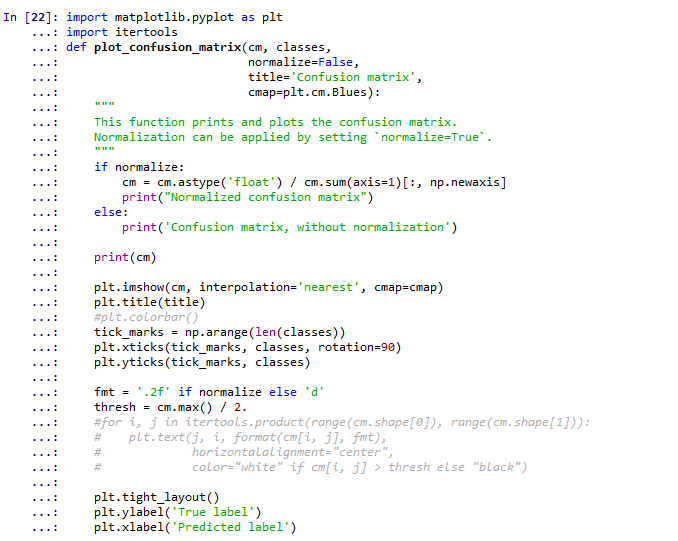
\includegraphics[width=4cm]{figures/1174054/3/27.png}
		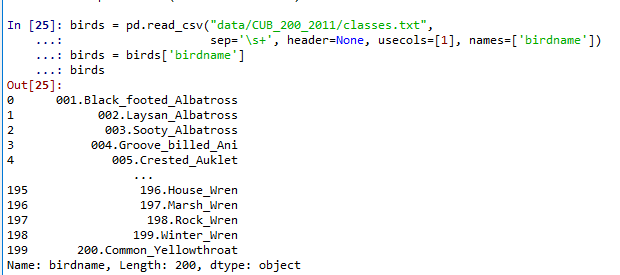
\includegraphics[width=4cm]{figures/1174054/3/28.png}
		\caption{Hasil Soal 5 - 3}
\end{figure}
\end{itemize}

\item Nomor 6
\hfill\break
\begin{itemize}
\item Menunjukkan klarifikasi dengan decission tree menggunakan dataset yang sama dan akan memunculkan akurasi prediksi.
\lstinputlisting[firstline=177, lastline=180]{src/1174054/3/1174054_teori.py}
Hasilnya:
\begin{figure}[H]
	\centering
		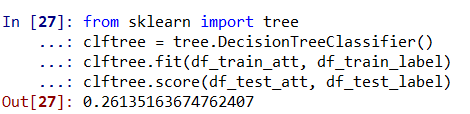
\includegraphics[width=4cm]{figures/1174054/3/29.png}
		\caption{Hasil Soal 6 - 1}
\end{figure}
		
\item Menunjukkan klarifikasi dengan SVM menggunakan dataset yang sama dan akan memunculkan akurasi prediksi.
\lstinputlisting[firstline=185, lastline=188]{src/1174054/3/1174054_teori.py}
Hasilnya:
\begin{figure}[H]
	\centering
		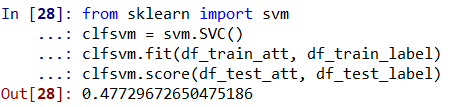
\includegraphics[width=4cm]{figures/1174054/3/30.png}
		\caption{Hasil Soal 6 - 2}
\end{figure}
\end{itemize}

\item Nomor 7
\hfill\break
\begin{itemize}
\item Menunjukkan hasil cross validation pada Random Forest.
\lstinputlisting[firstline=193, lastline=195]{src/1174054/3/1174054_teori.py}
Hasilnya:
\begin{figure}[H]
	\centering
		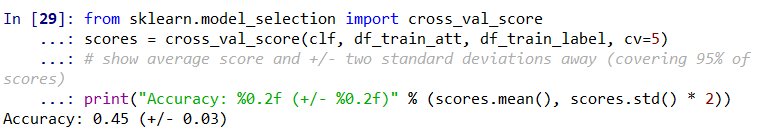
\includegraphics[width=4cm]{figures/1174054/3/31.png}
		\caption{Hasil Soal 7 - 1}
\end{figure}
		
\item Menunjukkan hasil cross validation pada Desiccion Tree.
\lstinputlisting[firstline=200, lastline=201]{src/1174054/3/1174054_teori.py}
Hasilnya:
\begin{figure}[H]
	\centering
		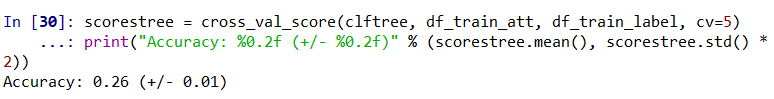
\includegraphics[width=4cm]{figures/1174054/3/32.png}
		\caption{Hasil Soal 7 - 2}
\end{figure}
		
\item Menunjukkan hasil cross validation pada SVM.
\lstinputlisting[firstline=206, lastline=207]{src/1174054/3/1174054_teori.py}
Hasilnya:
\begin{figure}[H]
	\centering
		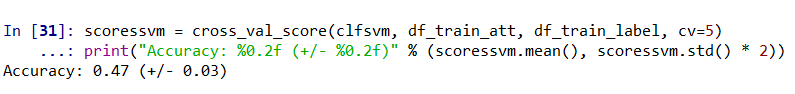
\includegraphics[width=4cm]{figures/1174054/3/33.png}
		\caption{Hasil Soal 7 - 3}
\end{figure}
\end{itemize}

\item Nomor 8
\begin{itemize}
\item Menunjukkan informasi-informasi tree yang dibuat.
\lstinputlisting[firstline=212, lastline=225]{src/1174054/3/1174054_teori.py}
Hasilnya:
\begin{figure}[H]
	\centering
		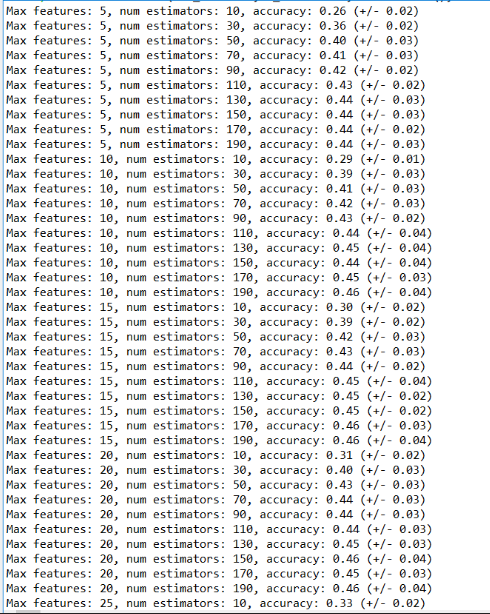
\includegraphics[width=4cm]{figures/1174054/3/34.png}
		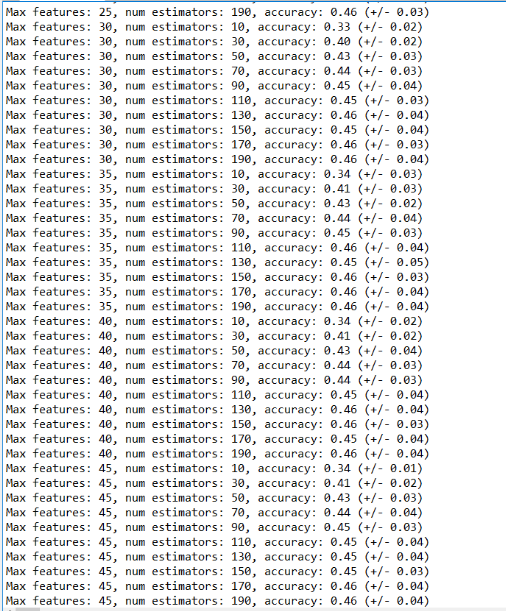
\includegraphics[width=4cm]{figures/1174054/3/35.png}
		\caption{Hasil Soal 8 - 1}
\end{figure}
		
\item Menunjukkan hasil dari plotting komponen informasi sehingga dapat kita baca sebagai grafik 3D.
\lstinputlisting[firstline=230, lastline=244]{src/1174054/3/1174054_teori.py}
Hasilnya:
\begin{figure}[H]
	\centering
		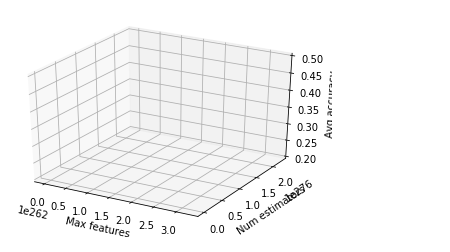
\includegraphics[width=4cm]{figures/1174054/3/36.png}
		\caption{Hasil Soal 8 - 2}
\end{figure}
\end{itemize}
\end{enumerate}

\subsection{Penanganan Error}
\begin{enumerate}
\item ScreenShoot Error
	\begin{figure}[H]
		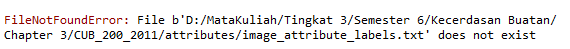
\includegraphics[width=4cm]{figures/1174054/3/error1.png}
		\centering
		\caption{File Not Found Error}
	\end{figure}

	\item Tuliskan Kode Error dan Jenis Error
	\begin{itemize}
		\item File Not Found Error

	\end{itemize}
	\item Cara Penanganan Error
	\begin{itemize}
		\item File Not Found Error
		\hfill\break
		Error terdapat pada kesalahan baca file csv, yang tidak terbaca. Dikarenakan letak file yang dibaca tidak para direktori yang sama. Seharusnya letakkan file di direktori yang sama. 
	\end{itemize}
\end{enumerate}

\subsection{Bukti Tidak Plagiat}
\begin{figure}[H]
	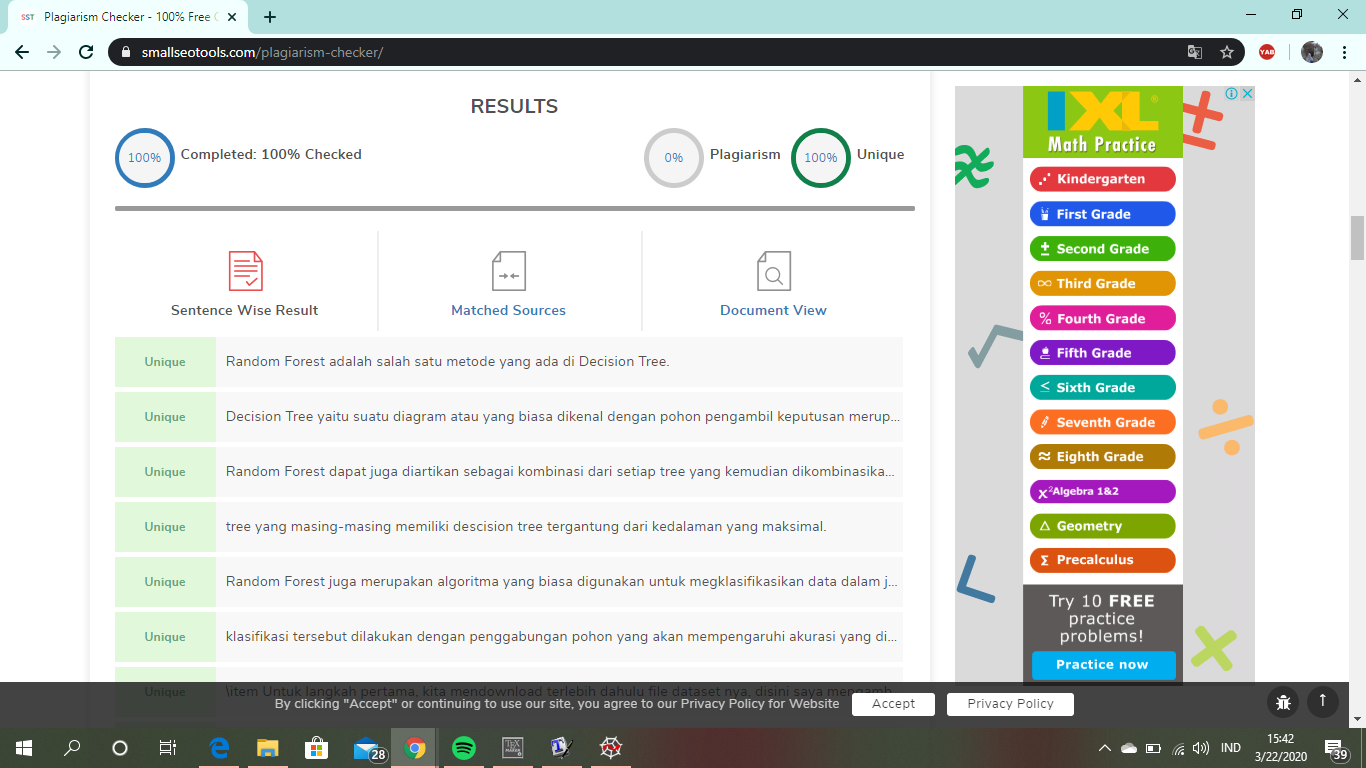
\includegraphics[width=4cm]{figures/1174054/3/plagiarisme.png}
	\centering
	\caption{Bukti Tidak Plagiat}
\end{figure}

\subsection{Link Youtube}
